\documentclass[UTF8]{article}
\usepackage[fontset=fandol]{ctex} % Chinese support, using Fandol fonts
\usepackage{graphicx} % Insert images
\usepackage{listings} % Print source code
\usepackage{xcolor} % Color support
\usepackage{booktabs} % Professional table support
\usepackage{pdflscape} % Landscape pages support in PDF
\usepackage{hyperref} % Hypertext links support for cross-referencing
\usepackage{geometry} % Page layout
\usepackage{enumitem} % Enumerate and itemize
\usepackage{setspace} % Set line spacing。

% Customize hyperref format (it's set to no special format here)
\hypersetup{hidelinks}

% Declare directories to search for graphics files for graphicx
\graphicspath{{figures/}}

% Set c style for lstlisting
\lstdefinestyle{c-style}{
  language=C,
  basicstyle=\ttfamily\small, % 基本字体样式和大小
  keywordstyle=\bfseries\color{blue!70!black}, % 关键字样式
  identifierstyle=\color{teal}, % 标识符样式
  stringstyle=\color{purple}, % 字符串样式
  commentstyle=\itshape\color{green!70!black}, % 注释样式
  backgroundcolor=\color{gray!10}, % 背景颜色
  numbers=left, % 行号在左边
  numberstyle=\tiny\color{gray}, % 行号字体样式
  numbersep=6pt, % 行号与代码间的距离
  breaklines=true, % 自动换行
  postbreak=\mbox{\textcolor{red}{$\hookrightarrow$}\space}, % 换行符号
  frame=single, % 单线框
  framerule=0.5pt, % 框线宽度
  rulecolor=\color{black}, % 框线颜色
  tabsize=4, % 制表符宽度
  captionpos=b, % 标题位置在下方
  showspaces=false, % 不显示空格
  showstringspaces=false, % 不显示字符串中的空格
  showtabs=false, % 不显示制表符
  morekeywords={*,printf,scanf}, % 更多关键字
  escapeinside={(*@}{@*)}, % 支持代码中插入LaTeX
  xleftmargin=2em, % 左侧边距
  xrightmargin=2em, % 右侧边距
  aboveskip=1em, % 代码块与上下文的间距
  belowskip=1em % 代码块与上下文的间距
}

% Define new command for title page
\newcommand{\reporttitle}[2]{
  \LARGE\textsf{#1}\quad\underline{\makebox[12em]{#2}}
}
\newcommand{\reportinfo}[2]{
  \large\makebox[4em]{\textsf{#1}}\quad\underline{\makebox[18em]{#2}}
}
\newcommand{\smallertitlefont}[2]{{\fontsize{#1}{1.2\baselineskip}\selectfont\mdseries #2}}
\newcommand{\smallermaintitlefont}[2]{{\fontsize{#1}{1.2\baselineskip}\selectfont\bfseries #2}}
\newcommand{\Modified}[1]{{}}
% \newcommand{\TODO}[1]{{}}
\newcommand{\Add}[1]{{}}
\newcommand{\TODO}[1]{\textbf{(TODO: {#1})}}

% ----- The document begins here -----
\begin{document}

% Title page
\title{ \bfseries{\Huge Hajimi-OS 作品文档}}
\author{\smallermaintitlefont{15pt}{队名:厚积薄发队}  \\[10pt] \smallertitlefont{12pt}{\textbf{团队成员:邹扬,夏彦文,雷翔麟  }}
  \\[10pt] \smallertitlefont{12pt}{\textbf{指导老师:潘鹏  }}
  \\[320pt] \smallertitlefont{12pt}{\textbf{计算机科学与技术学院}}
  \\[10pt] \smallertitlefont{12pt}{\textbf{华中科技大学}}
}

% \author{\smallermaintitlefont{15pt}{邹扬,夏彦文,雷翔麟}}
% \author{夏彦文 \thanks{学生,计算机学院数据科学与大数据} \and 雷翔麟 \thanks{学生,计算机科学与技术学院}
%   \and 邹扬 \thanks{学生,计算机学院数据科学与大数据} \and 潘鹏 \thanks{指导教师,计算机科学与技术学院}}
% \institution{Huazhong University of Science and Technology}
\date{\today}
\maketitle

% Table of contents
\setstretch{1.1} % 刚好能让目录在一页内
\newpage
\tableofcontents
\newpage

% 设定1.6倍行距
\setstretch{1.6}

% Main content
\section{介绍}
Hajimi-OS 是一款面向现代计算需求而设计的操作系统,运行在 RISC-V 架构上。它不仅仅是一个操作系统,而是一个通过整合前沿技术、提升系统性能和安全性,为用户提供全新计算体验的创新项目。Hajimi-OS 的设计理念来自于多种经典操作系统的精华,并结合了当前计算领域的发展趋势和需求。

\subsection{作品意义与背景}
在当今信息化社会,操作系统作为计算机系统的核心,其重要性不言而喻。操作系统不仅管理硬件资源,还为应用程序提供运行环境和接口。随着物联网、大数据和人工智能等新兴技术的发展,传统的操作系统面临着性能、安全性和扩展性的多重挑战。

Hajimi-OS 的开发背景源于对现有操作系统在面对新技术需求时的不足进行改进。通过模块化设计和微内核架构,Hajimi-OS 力图在保持高效性和稳定性的同时,提供更强的兼容性和扩展性。我们的目标是打造一个灵活、安全且高效的操作系统,以应对未来的计算挑战。

项目的意义在于:
\begin{itemize}
  \item 提升计算机教育质量:当前的计算机教育中,理论与实践的结合尚有不足。通过 Hajimi-OS,我们希望提供一个完整的操作系统开发实验平台,使学生能够深入理解操作系统的核心概念和实现机制,从而提升他们的实践能力和理论理解。
  \item 推动操作系统技术进步:Hajimi-OS 采用了许多前沿技术和设计理念,如 RISC-V 架构、微内核设计等。通过这一项目,我们希望为操作系统领域带来新的思路和突破,推动技术的不断进步。
  \item 增强系统安全性和性能:面对日益严峻的网络安全威胁和不断增长的计算需求,Hajimi-OS 在安全性和性能优化方面进行了大量创新设计,旨在提供一个更加安全、高效的操作系统环境。
  \item 促进自主创新和开源合作:通过开源社区的合作,我们希望推动操作系统技术的共享和创新。
\end{itemize}

\subsection{国内外研究状况}
操作系统内核是操作系统的核心部分,负责处理硬件与软件之间的交互。国内外在操作系统内核的研究方面已经取得了大量成果,从商业系统到开源系统,都有许多成功的案例和研究方向。

在商业操作系统方面:
\begin{itemize}
  \item 微软 Windows:微软的 Windows 操作系统使用的是 NT 内核,这是一种混合内核,结合了微内核和宏内核的特点。微软投入了大量资源进行 NT 内核的研发,以提供高效、安全和稳定的用户体验。
  \item 苹果 macOS:苹果的 macOS 使用的是 XNU 内核,这也是一种混合内核,包含了 Mach 微内核和 BSD 宏内核的部分。苹果在提高性能、增强安全性和支持新硬件方面做了大量工作。
\end{itemize}

在开源操作系统方面:
\begin{itemize}
  \item Linux:Linux 内核是一个开源的宏内核项目,全球有数万名开发者参与其中。Linux 内核被广泛应用于服务器、超级计算机、嵌入式设备和个人桌面环境。中科院软件研究所和哈工大等国内机构也在进行基于 Linux 内核的操作系统研究,如可信鸿蒙和麒麟操作系统,分别针对网络安全和国产化需求进行优化。
\end{itemize}

在未来操作系统的研究趋势中:
\begin{itemize}
  \item 微内核:微内核通过将大部分功能移到用户空间,提高了系统的可靠性和安全性。Google 的 Fuchsia 操作系统使用的 Zircon 微内核就是一个典型例子。
  \item 安全性:随着网络安全问题的日益突出,内核自我保护、内核隔离和内核加固等技术成为当前的研究重点。
  \item 新硬件支持:随着多核处理器、非易失性内存和量子计算机等新硬件的发展,如何更好地利用这些硬件也是操作系统研究的重要方向。
\end{itemize}

\subsection{主要工作}
Hajimi-OS 项目作品的开发工作涵盖了从内核设计到用户界面的一系列任务,具体包括以下几个方面:

\begin{itemize}
  \item 系统架构设计:Hajimi-OS 采用模块化和微内核设计,将操作系统的核心功能最小化,并将其他服务模块化,以提高系统的灵活性和安全性。系统架构包括内核层、服务层和应用层,各层之间通过定义明确的接口进行通信。
  \item 内核开发:内核是操作系统的核心,负责管理硬件资源和提供基础服务。Hajimi-OS 的内核开发包括进程管理、内存管理、设备驱动、文件系统和网络协议等模块。我们采用现代编程技术和工具,确保内核的高效性和可靠性。
  \item 硬件抽象接口 SBI:我们开发了一套全新的中断处理机制,适应不同硬件平台的特性,更有效地处理和分发中断。我们还开发了无效指令软处理机制,在软件层面扩展硬件功能,提高操作系统的兼容性和扩展性。
  \item 用户抽象接口 ABI:增加了新的系统调用,使用户程序可以更方便地使用操作系统提供的服务。这些系统调用覆盖文件操作、进程管理和内存管理等多个领域,支持更复杂的用户程序。
  \item 性能优化:优化内核的调度算法,使系统可以更公平、高效地分配 CPU 时间。改进内核的内存管理,提高系统在各种使用场景下的响应速度和资源利用率。
  \item 丰富文档:提供详尽的开发文档和用户手册,帮助用户和开发者快速上手。
\end{itemize}

Hajimi-OS 致力于为用户提供高性能、高安全性且用户友好的操作系统。我们希望通过这一项目,不仅为用户提供更好的计算体验,也为操作系统技术的发展贡献力量。未来,我们将继续完善和优化 Hajimi-OS,探索更多前沿技术,并与学术界和工业界的伙伴们合作,共同推动操作系统领域的创新和进步。

\section{理念与目标}
在 Hajimi-OS 项目的开发过程中,我们设定了实现一系列系统调用的目标,以满足操作系统的基本功能需求。系统调用是操作系统与应用程序之间的接口,提供了执行各种操作的基本功能。在操作系统的设计与实现过程中,为了确保系统的功能完备性和稳定性,我们依据具体需求定义了一组系统调用编号。这些编号不仅涵盖了基本的操作系统功能,还包括了一些增强功能,以支持更多的应用场景和操作。

我们定义了如下系统调用编号:
\lstinputlisting[style=c-style]{syscallnumber.c}

为了充分支持操作系统的功能性评测,我们需要确保系统能够处理这些调用,并且提供必要的扩展性。Hajimi-OS 不仅要支持这些标准系统调用,还要提供一些额外的功能,如增强的文件系统支持、进程管理功能等。这些系统调用的设计和实现体现了我们对操作系统功能和性能的高标准要求,以及对未来扩展性和灵活性的前瞻性考虑。通过这样精心设计的系统调用,我们希望 Hajimi-OS 能够在多种应用场景中表现出色,为用户提供稳定、高效的操作体验。

\section{设计与实现}
\subsection{进程管理}
进程管理模块的主要功能包括:初始化进程、加载和解析进程、切换进程,以及构建进程状态模块。具体功能介绍如下。
\subsubsection{进程控制块}
进程作为操作系统提供的一种抽象层,实际上代表了正在执行的程序。为了便于管理进程,Hajimi-OS采用进程控制块\texttt{PCB}来管理操作系统的进程。进程控制块的结构如下所示。
进程控制块中包含了进程的状态信息,这是操作系统管理进程的基本单元。关于具体的状态,我们将在后文详细解析。
\lstinputlisting[style=c-style]{processblock.c}
\subsubsection{进程状态}
进程状态是一个枚举类型,其定义如下:
\lstinputlisting[style=c-style]{processstate.c}
各状态对应如下:
\begin{enumerate}[label=\textbf{\arabic*}., wide, labelwidth=!, labelindent=0pt]
  \item UNUSED 状态表示进程控制块未关联任何进程。
  \item SLEEPING 状态表示进程因某种原因暂时未运行。
  \item RUNNABLE 状态表示进程正等待调度器安排运行
  \item RUNNING 状态表示进程正在执行中。
  \item ZOMBIE 状态表示进程已终止,但资源尚未被回收。
\end{enumerate}
\subsubsection{分配进程}
在 Hajimi-OS 中,分配新进程的过程由 \texttt{allocproc} 函数负责。这个函数主要执行以下步骤:
\begin{enumerate}[label=\textbf{\arabic*}., wide, labelwidth=!, labelindent=0pt]
  \item \textbf{查找 UNUSED 状态的进程控制块:} 系统首先会扫描进程控制块数组,寻找一个状态为 \texttt{UNUSED} 的控制块。如果找到,程序跳转到 \texttt{found} 标签继续操作;如果未找到,则返回 \texttt{NULL},表示当前没有可用的进程控制块,无法创建新进程。
  \item \textbf{初始化进程控制块:} 找到未使用的进程控制块后,函数会分配一个新的进程 ID(通过调用 \texttt{allocpid} 函数) ,将虚拟内存地址\texttt{vma}设置为 \texttt{NULL},并将内核时间\texttt{ktime}和用户时间\texttt{utime}初始化为 1。
  \item \textbf{分配 trapframe 页面:} 函数为新进程的 \texttt{trapframe} 分配内存(通过调用 \texttt{kalloc} 函数)。如果内存分配失败,函数将释放进程锁并返回 \texttt{NULL}。
  \item \textbf{创建用户和内核页表:} 成功分配 \texttt{trapframe} 页面后,函数创建一个空的用户页表(通过调用 \texttt{proc\_pagetable} 函数)和一个内核页表(通过调用 \texttt{proc\_kpagetable} 函数)。如果任一页表创建失败,函数会清理进程资源并返回 \texttt{NULL}。
  \item \textbf{配置内核堆栈\texttt{kstack}:} 成功分配页表后,函数会设置进程的内核堆栈地址,该地址是预设的虚拟地址。
  \item \textbf{设置新进程的上下文:} 函数初始化进程的上下文\texttt{context},将返回地址寄存器\texttt{ra}设为 \texttt{forkret} 函数地址,堆栈指针\texttt{sp}设为内核堆栈顶部。如此设置后,新进程将从 \texttt{forkret} 函数开始执行。
\end{enumerate}
通过这些步骤,\texttt{allocproc} 函数完成了新进程的创建。每个新创建的进程在完成这些步骤后,都会拥有一个唯一的进程 \texttt{ID},以及自己的页表和堆栈,准备好开始执行。
\subsubsection{加载和解析进程}
在 Hajimi-OS 中,除 \texttt{init} 进程外,所有进程都是通过 \texttt{fork} 系统调用进行复制,然后使用 \texttt{exec} 系统调用加载新程序来执行的。
对于 \texttt{init} 进程,初始化过程如下:
\begin{enumerate}[label=\textbf{\arabic*}., wide, labelwidth=!, labelindent=0pt]
  \item \textbf{进程分配:} Hajimi-OS 预设了固定数量的进程控制块 \texttt{Process Control Block}。每次创建新进程时,系统会在 \texttt{PCB} 数组中寻找一个空闲的块。
  \item \textbf{页表映射:} Hajimi-OS 使用 \texttt{RISC-V} 的 \texttt{sv39} 虚拟内存模型。在此步骤中,操作系统会为程序的各个段(如代码段、数据段等)进行页表映射。我们预先编译了一段二进制代码,专门用于执行 \texttt{init} 程序。 \texttt{init} 程序将使用 \texttt{fork} 系统调用创建一个新进程,然后通过 \texttt{exec} 系统调用执行 \texttt{shell} 程序。原始的 \texttt{init} 进程则会进入无限的进程调度循环。
  \item \textbf{设置进程状态:} 完成以上步骤后,操作系统将进程状态设置为 \texttt{RUNNABLE}。
\end{enumerate}
代码如下:
\lstinputlisting[style=c-style]{processinit.c}
对于其他进程,其初始化过程大致如下:
\begin{enumerate}[label=\textbf{\arabic*}., wide, labelwidth=!, labelindent=0pt]
  \item \textbf{使用 \texttt{fork} 系统调用:} \texttt{fork} 的主要功能是生成一个与父进程完全相同的子进程。这个过程包括为新进程创建一个进程控制块\texttt{PCB},复制父进程的页表,并在 \texttt{PCB} 中记录父子进程关系,具体存储在 \texttt{PCB} 的 \texttt{parent} 字段中。
  \item \textbf{执行 \texttt{exec} 系统调用:} \texttt{exec} 的主要作用是解析 \texttt{ELF} 文件,并为进程重新映射虚拟内存。通过这种方式,新程序能够在原进程的环境中运行,而不仅仅是复制父进程的行为。这个过程确保了进程的正确创建和程序的正确加载,保证了 Hajimi-OS 的多进程环境能够正常运行。
\end{enumerate}

\subsubsection{进程调度}
目前,texttt{Hajimi-OS} 操作系统采用时间片均分策略进行进程调度。因此,在时钟中断时,操作系统会中断当前进程并调度下一个进程执行。所有进程的优先级相同,统一放在一个队列中进行调度。接下来,我们将介绍进程切换过程,但首先需要了解 Hajimi-OS 对 CPU 的抽象。

在 Hajimi-OS 中,\texttt{CPU} 由以下结构体管理,其中关键字段是 \texttt{proc} 和 \texttt{context}。\texttt{proc} 字段指向当前在该 \texttt{CPU} 上运行的进程,而 \texttt{context} 字段用于进程切换。
\lstinputlisting[style=c-style]{cpustruct.c}
context 的定义如下:
\lstinputlisting[style=c-style]{contextstruct.c}
context 用于保存当前进程的上下文,以便进程下次运行时恢复。Hajimi-OS 的进程调度通过 \texttt{scheduler} 函数实现,当系统需要进行进程切换时,它会扫描所有进程,寻找状态为 RUNNABLE 的进程。

首先,\texttt{scheduler} 函数从进程列表中选择一个状态为 RUNNABLE 的进程。获取进程后,会锁定该进程以防止其他进程同时修改其状态。

接下来,将选中的 RUNNABLE 进程状态改为 RUNNING,并将其设置为当前 CPU 正在运行的进程。此时,函数会切换页表到选中进程的内核页表,并刷新地址空间。

然后,函数执行 \texttt{swtch} 操作,将当前 CPU 的 context 与待运行进程的 context 进行切换。此操作涉及更改处理器的 ra 和 sp 寄存器,使处理器跳转到新进程指定的地址执行,即待运行进程的 ra 寄存器地址。当进程运行结束后,处理器会返回到 \texttt{scheduler} 函数,并将页表切换回内核页表,同时刷新地址空间。此时,进程状态可能已发生变化。

最后,当前 CPU 的正在运行进程被设置为 0,表示 CPU 暂时没有正在运行的进程。然后释放进程的锁,进行下一轮进程选择。

如果在一轮循环中没有找到可运行的进程,系统将执行 \texttt{wfi} 指令使处理器进入休眠状态,等待中断唤醒。

\subsubsection{进程释放}
在 Hajimi-OS 中,当一个进程结束或在进程创建过程中发生错误时,需要释放该进程所占用的资源,这个过程通过 freeproc 函数来完成。该函数的主要步骤如下:
\begin{enumerate}[label=\textbf{\arabic*}., wide, labelwidth=!, labelindent=0pt]
  \item \textbf{释放 \texttt{trapframe}:} 首先,如果 \texttt{trapframe} 存在,则释放其占用的内存,并将 \texttt{trapframe} 字段设为 0。
  \item \textbf{释放内核页表:} 如果内核页表\texttt{kpagetable}存在,则释放其占用的内存,然后将 \texttt{kpagetable} 字段设为 0。
  \item \textbf{释放用户页表:} 如果用户页表\texttt{pagetable}存在,利用 \texttt{proc\_freepagetable} 函数释放用户页表所占用的内存,同时将 \texttt{pagetable} 字段设为 0。
  \item \textbf{清空进程控制块的其他字段:} 清空进程的虚拟内存地址\texttt{vma},将进程大小\texttt{sz}设为 0,进程 ID\texttt{pid}设为 0,父进程\texttt{parent}设为 0,清空进程的名称\texttt{name},清空等待的条件变量\texttt{chan},设置进程未被杀死(将 \texttt{killed} 设为 0),并将进程的扩展状态设为 0。
  \item \textbf{设置进程状态为 \texttt{UNUSED}:} 最后,将进程状态设为 \texttt{UNUSED},表示该进程控制块可以重新分配给新的进程使用。
\end{enumerate}
通过这些步骤,\texttt{freeproc} 函数实现了对进程资源的回收,包括内存资源(如 trapframe、页表等)和进程控制块中的各种字段。回收完毕后,该进程控制块即可被系统重新利用,用于创建新的进程。

\subsection{内存管理}
\subsubsection{物理内存管理}
物理内存管理是操作系统的核心部分之一。Hajimi-OS 采用了一种简单且高效的物理内存分配和回收算法,主要由 kalloc.c 模块负责。该模块实现了初始化物理内存、分配物理内存和回收物理内存的功能。

\paragraph{内存管理概述\\}
在 Hajimi-OS 中,物理内存是按页进行管理的,每页大小为 4096 字节。系统中的所有空闲物理内存页通过一个单向链表组织起来,链表中的每个节点代表一个物理内存页。以下是相关数据结构和变量:
\begin{enumerate}[label=\textbf{\arabic*}., wide, labelwidth=!, labelindent=0pt]
  \item \textbf{struct run}: 这是一个简单的链表节点结构,表示一个空闲的物理内存页,next 指针指向下一个空闲内存页。
        \lstinputlisting[style=c-style]{runstruct.c}
  \item \textbf{kmem}: 这是一个全局变量,用于管理所有的空闲物理内存页。texttt{freelist} 指针指向空闲内存页链表的头部,\texttt{npage} 记录当前系统中空闲物理内存页的数量。\texttt{kmem} 中还包含一个名为 \texttt{lock} 的自旋锁,用于在多核环境下保护内存分配和回收操作的原子性。
        \lstinputlisting[style=c-style]{kmemstruct.c}
\end{enumerate}

\paragraph{核心函数}
\begin{enumerate}[label=\textbf{\arabic*}., wide, labelwidth=!, labelindent=0pt]
  \item \texttt{kfree} 该函数用于释放一个物理内存页,接收一个指向物理内存页的指针。函数首先检查传入的物理地址是否合法,然后将该物理内存页的内容清空,并将其添加到空闲内存页链表的头部。
        \lstinputlisting[style=c-style]{kfree.c}
  \item \texttt{kalloc} 该函数用于释放一个物理内存页,接收一个指向物理内存页的指针。函数首先检查传入的物理地址是否合法,然后将该物理内存页的内容清空,并将其添加到空闲内存页链表的头部。
        \lstinputlisting[style=c-style]{kalloc.c}
  \item \texttt{kinit} 该函数在系统启动时调用,用于初始化物理内存管理系统。它首先初始化 \texttt{kmem} 中的自旋锁,然后调用 \texttt{freerange} 函数,将从内核结束地址 \texttt{kernel\_end} 到物理内存上限 \texttt{PHYSTOP} 之间的所有物理内存页添加到空闲列表中。
        \lstinputlisting[style=c-style]{kinit.c}
  \item \texttt{freerange} 此函数用于将一段物理内存地址范围内的所有物理内存页释放,并加入到空闲内存页链表中。它首先将起始地址向上取整到页的边界,然后从起始地址开始,每次增加一个页的大小(4096 字节),依次释放每个物理内存页。
        \lstinputlisting[style=c-style]{freerange.c}
  \item \texttt{freemem\_amount} 此函数返回当前系统中的空闲物理内存量。由于内存页的大小是固定的,所以直接将空闲内存页的数量左移 12 位即可得到空闲内存的字节数。
        \lstinputlisting[style=c-style]{freemem_amount.c}
\end{enumerate}


\paragraph{设计评价与改进方向\\}
Hajimi-OS 的物理内存管理通过单一链表管理所有空闲内存页,采用简单的链表操作实现物理内存页的分配和回收,满足了操作系统对物理内存管理的基本需求。然而,未来可以考虑以下改进方向:
\begin{enumerate}[label=\textbf{\arabic*}., wide, labelwidth=!, labelindent=0pt]
  \item \textbf{支持大页分配:} 当前实现只支持分配和回收固定大小的内存页。如果需要分配大块的连续物理内存,需要进行多次分配操作,可能影响性能。可以考虑支持大页的分配,以提高内存访问的性能。
  \item \textbf{改进内存分配策略:} 目前的实现采用简单的“先进先出”策略分配内存页,可能导致物理内存的使用分布不均。可以考虑引入更复杂的内存分配策略,如伙伴系统(\texttt{Buddy System})或者 \texttt{slab} 分配器。
  \item \textbf{改进锁机制:} 当前实现中,所有对物理内存的操作都需要获取全局的 \texttt{kmem} 锁,这在多核环境下可能成为性能瓶颈。可以考虑引入更细粒度的锁机制,如每个 \texttt{CPU} 拥有自己的内存池和锁,或者使用无锁数据结构来提高并发性。
\end{enumerate}

\subsubsection{虚拟内存管理}

\paragraph{Hajimi-OS 虚拟内存管理\\}
页表是虚拟内存管理的重要工具。在 Hajimi-OS 中,运行在 RISC-V 的 Sv39 配置下,这意味着在 64 位虚拟地址中,只有低 39 位被使用,高 25 位闲置。Sv39 模式下,RISC-V 页表在逻辑层面上看似包含 2\textsuperscript{27} 个页表条目 PTE。每个 PTE 由 44 位的物理页码 PPN 和若干标志位组成。分页硬件利用虚拟地址的前 27 位索引页表,生成的物理地址为 56 位,其前 44 位来自 PTE 中的 PPN,后 12 位直接来自虚拟地址。

\paragraph{页表结构与地址转换\\}
页表逻辑上是一个简单的 PTE 数组(见图 3.2)。页表允许操作系统控制虚拟地址到物理地址的映射,以 4096 字节(2\textsuperscript{12} 字节)为单位。在 Sv39 配置下,虚拟地址的前 25 位不参与地址转换;未来 RISC-V 设计中,这些位可能用于更多级别的地址转换。此外,物理地址的扩展空间也预留了 10 位以便扩展物理地址长度。基于技术预测,2\textsuperscript{39} 字节(512GB)的虚拟内存空间能满足 RISC-V 计算机应用的需求,物理内存空间的 2\textsuperscript{56} 字节也足以支持未来的 I/O 设备和 DRAM 需求。

地址转换是一个三步过程。页表在物理内存中以三层树状结构存储,根节点为一个 4096 字节的页表页面,包含 512 个 PTE。每个 PTE 记录了下一层页表页的物理地址。分页硬件依次利用虚拟地址的 27 位选择 PTE:前 9 位用于根页表页面,中间 9 位用于中间页表页面,最后 9 位用于最终页表页面。若缺少任何一个必要的 PTE,分页硬件会抛出页面错误异常,Hajimi-OS 负责处理该异常。

\paragraph{页表条目 PTE 与硬件缓存\\}
三级设计在许多虚拟地址范围未映射的情况下节省内存。例如,一个应用程序仅使用一个页面,顶级页目录仅使用第 0 个条目,忽略第 1 到第 511 个条目,无需为这些条目分配中级和低级页表页。该设计在这种情况下仅占用三个页面,总共 3 × 4096 字节。然而,CPU 在执行地址转换时必须从内存中提取三个 PTE,从而增加了内存访问的开销。为降低 PTE 加载成本,RISC-V CPU 将页表条目缓存在 Translation Look-aside Buffer中。

每个 PTE 包含若干标志位,指示分页硬件如何处理对应的虚拟地址:
\begin{enumerate}[label=\textbf{\arabic*}., wide, labelwidth=!, labelindent=0pt]
  \item PTE\_V:PTE 是否存在,未设置则引用页面引发异常。
  \item PTE\_R:是否允许读取页面。
  \item PTE\_W:是否允许写入页面。
  \item PTE\_X:是否允许执行页面内容。
  \item PTE\_U:用户模式下是否可访问页面。
\end{enumerate}
\lstinputlisting[style=c-style]{riscv.c}
这些标志位和结构在 \texttt{kernel\textbackslash include\textbackslash sys\textbackslash riscv.h} 中定义。

\paragraph{Hajimi-OS 虚拟内存管理代码\\}
虚拟内存管理系统主要负责分页和内存映射。关键函数包括:
\begin{enumerate}[label=\textbf{\arabic*}., wide, labelwidth=!, labelindent=0pt]
  \item \textbf{\texttt{kvminit()}:} 创建一个直接映射的页表用于内核,设置不同设备和内核区域的映射。
  \item \textbf{\texttt{kvminithart()}:} 设置硬件的页表寄存器为内核页表并启用分页。
  \item \textbf{\texttt{walk()}:} 返回对应给定虚拟地址的 PTE 地址,必要时创建页表页。
  \item \textbf{\texttt{walkaddr()}:} 返回给定虚拟地址对应的物理地址,未映射则返回 0。
  \item \textbf{\texttt{kvmmap()}:} 向内核页表添加映射,用于启动时,不刷新 TLB。
  \item \textbf{\texttt{kvmpa()}:} 将内核虚拟地址转换为物理地址,用于栈地址。
  \item \textbf{\texttt{mappages()}:} 创建页表条目,映射从 \texttt{va} 开始的虚拟地址到 \texttt{pa} 开始的物理地址。
  \item \textbf{\texttt{vmunmap()}:} 移除从 \texttt{va} 开始的 \texttt{npages} 页的映射,必要时释放物理内存。
  \item \textbf{\texttt{uvmcreate()}:} 创建空用户页表,内存不足时返回 0。
  \item \textbf{\texttt{uvminit()}:} 将用户初始代码加载到页表地址 0,用于第一个进程。
  \item \textbf{\texttt{uvmalloc1()}:} 虚拟地址 \texttt{start} 到 \texttt{end} 分配 PTE 和物理内存,成功返回 0 失败返回 -1。
  \item \textbf{\texttt{freewalk()}:} 遍历页表并递归释放所有子页表。
  \item \textbf{\texttt{uvmfree()}:} 释放用户内存页和页表页。
  \item \textbf{\texttt{uvmcopy()}:} 复制父进程页表及其物理内存到子进程页表。
  \item \textbf{\texttt{uvmclear()}:} 将指定虚拟地址的页表条目标记为用户无法访问。
  \item \textbf{\texttt{copyout()}:} 从内核复制数据到用户空间。
  \item \textbf{\texttt{copyout2()}:} 简化版 \texttt{copyout},直接在虚拟地址空间操作。
  \item \textbf{\texttt{copyin()}:} 从用户空间复制数据到内核。
  \item \textbf{\texttt{copyin2()}:} 简化版 \texttt{copyin},直接在虚拟地址空间操作。
  \item \textbf{\texttt{copyinstr()}:} 从用户空间复制以 null 结尾的字符串到内核空间。
  \item \textbf{\texttt{copyinstr2()}:} 简化版 \texttt{copyinstr},直接在虚拟地址空间操作。
  \item \textbf{\texttt{proc\_kpagetable()}:} 初始化每个进程的内核页表。
  \item \textbf{\texttt{kfreewalk()}:} 释放页表的内核空间。
  \item \textbf{\texttt{kvmfreeusr()}:} 释放用户页表的内核空间。
  \item \textbf{\texttt{kvmfree()}:} 释放整个内核页表。
  \item \textbf{\texttt{vmprint()}:} 打印页表的详细信息。
  \item \textbf{\texttt{experm()}:} 改变指定虚拟地址的页表条目的权限。
\end{enumerate}

\paragraph{虚拟内存管理设计\\}
Hajimi-OS 的分页系统将物理内存和虚拟内存划分为固定大小的页,通过页表进行映射。页表条目包含页的权限标志位和物理地址。多个函数用于遍历和修改页表,例如 \texttt{walk} 函数查找特定 \texttt{PTE},\texttt{mappages} 函数修改页表以映射虚拟地址到物理地址。\texttt{freewalk} 函数递归释放页表页,\texttt{uvmfree} 函数释放用户内存页和页表页。\texttt{uvmcopy} 负责从父进程页表复制内存到子进程页表,实现进程创建。\texttt{copyin} 和 \texttt{copyout} 实现内核与用户空间之间的数据复制。\texttt{experm} 函数修改页表条目的权限,\texttt{vmunmap} 函数取消页表中虚拟地址的映射。

Hajimi-OS 进程拥有独立页表,映射其虚拟地址空间到物理内存。操作系统在进程切换时也会切换页表,确保正确的地址映射。每个进程的用户内存从虚拟地址 \texttt{0} 开始,可增长至 \texttt{MAXVA}(定义于 \texttt{riscv.h}),内存寻址空间可达 \texttt{256GB}。独立页表和虚拟地址空间切换实现了进程隔离和内存地址映射,确保每个进程拥有独立的内存空间,同时提供灵活性和可扩展性,满足不同应用需求。

当进程请求更多用户内存时,Hajimi-OS 首先使用 \texttt{kalloc} 分配物理页面,再将相应的 \texttt{PTE} 添加到进程页表中,指向新分配的物理页面,并设置 \texttt{PTE} 标志位以指示页面的读写、执行和用户访问权限。大多数进程不使用整个用户地址空间,Hajimi-OS 在未使用的页表项中将 \texttt{PTE\_V} 标志设置为空闲状态。

页表的典型使用示例包括:不同进程的页表将用户地址转换为不同物理内存页面,使每个进程拥有独立的私有内存空间;每个进程看到的用户内存空间以虚拟地址 0 开始,可为非连续的物理内存;内核在用户地址空间顶部映射一个包含蹦床代码的页面,使所有进程地址空间均可访问同一物理页面。

% 插入展示图片
\begin{figure}[htbp]
  \centering
  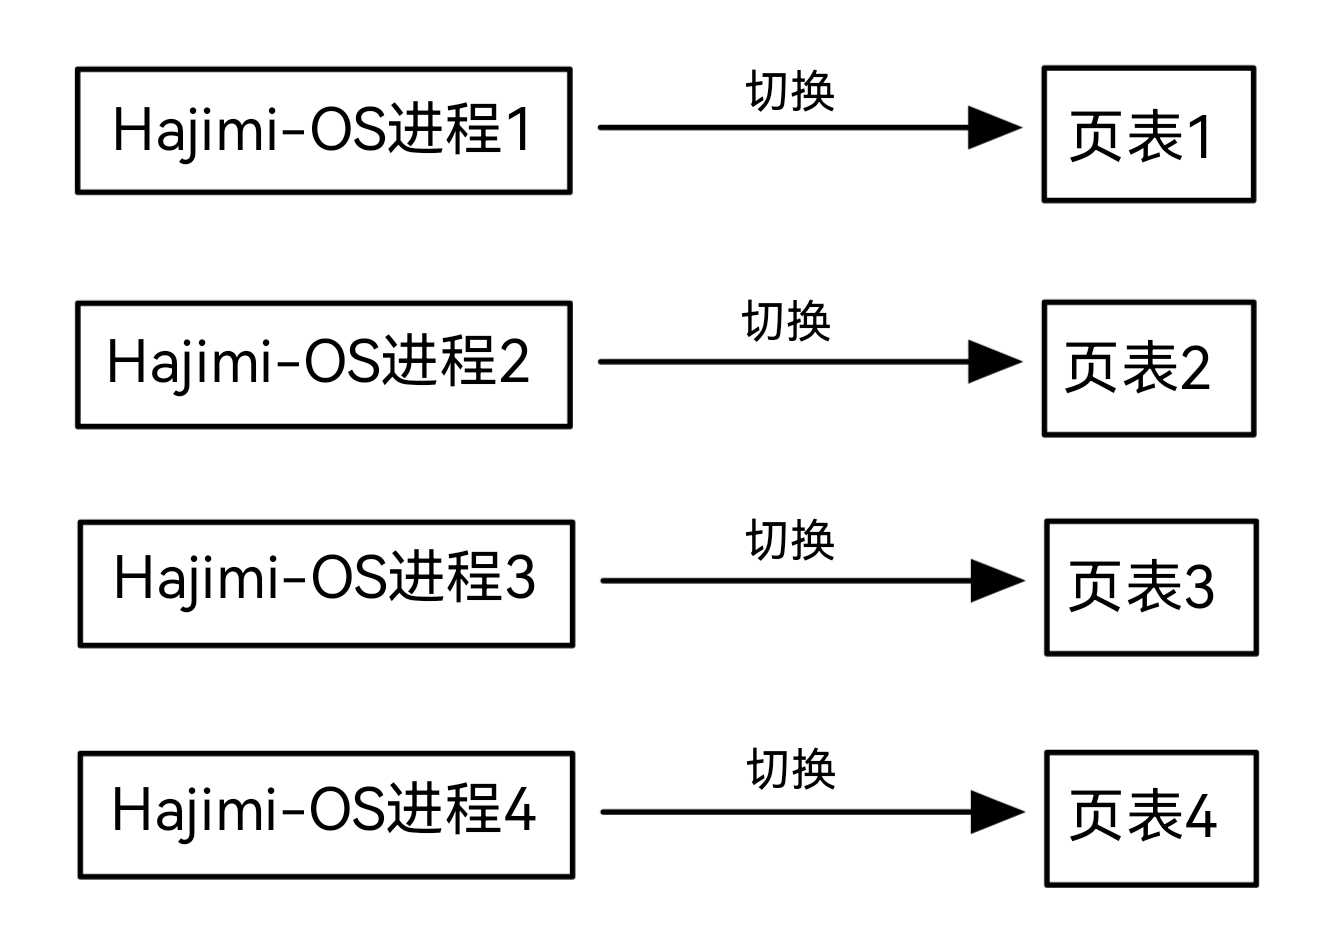
\includegraphics[width=0.8\textwidth]{mm1.png}
  \caption{进程页表}
  \label{进程页表}
\end{figure}
\begin{figure}[htbp]
  \centering
  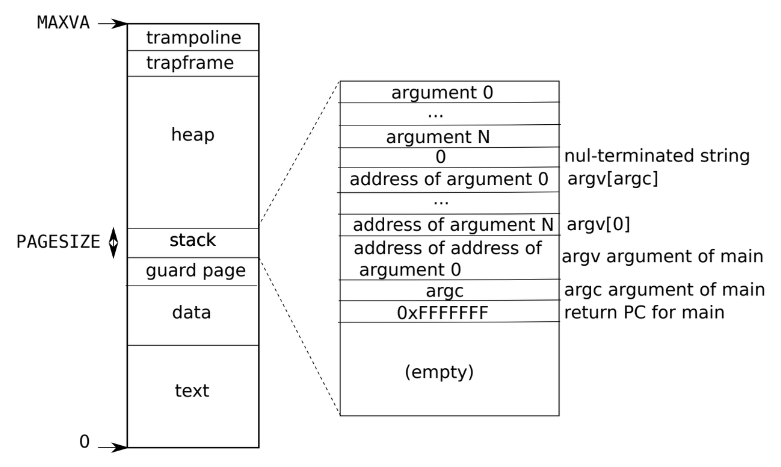
\includegraphics[width=0.8\textwidth]{mm2.png}
  \caption{地址空间}
  \label{地址空间}
\end{figure}

\paragraph{栈管理与保护\\}
在 Hajimi-OS 中,栈被分配为单独的页面,并在 \texttt{exec} 系统调用后初始化。栈的顶部包含命令行参数字符串及其指针数组,栈下方则包含启动程序所需的值,例如 \texttt{main} 函数的地址、\texttt{argc} 和 \texttt{argv} 参数。这样设计使程序如同刚刚调用 \texttt{main(argc, argv)} 一样开始执行。为了检测用户栈溢出,Hajimi-OS 在栈下方放置了一个无效的保护页(guard page)。如果用户栈溢出并尝试使用栈下方地址,由于该地址的页表项无效(\texttt{PTE\_V} 为 0),硬件会产生页面故障异常。当用户栈溢出时,操作系统可能会自动分配更多内存来避免问题。

\subsubsection{未来改进方向}
\paragraph{内存保护和安全性增强}
引入更多内存保护机制,以提高系统安全性
\begin{enumerate}[label=\textbf{\arabic*}., wide, labelwidth=!, labelindent=0pt]
  \item \textbf{内存隔离}: 确保不同进程间的内存隔离,防止越权访问。
  \item \textbf{内存清零}: 在内存释放或重分配时,将其内容清零,以防止数据泄露。
\end{enumerate}

\paragraph{高级内存管理功能}
为进一步优化内存使用,可以考虑引入高级内存管理技术
\begin{enumerate}[label=\textbf{\arabic*}., wide, labelwidth=!, labelindent=0pt]
  \item \textbf{\texttt{内存压缩:}} 通过压缩内存数据,提高内存利用率。
  \item \textbf{\texttt{NUMA 感知:}} 优化多处理器系统中的内存访问,以减少延迟。
  \item \textbf{\texttt{内存池预分配:}} 预先分配内存池以减少内存分配开销。
\end{enumerate}

\paragraph{增加缓存或预取机制}
通过预读取和缓存,提高内存访问速度
\begin{enumerate}[label=\textbf{\arabic*}., wide, labelwidth=!, labelindent=0pt]
  \item \textbf{\texttt{缓存机制:}} 在硬件或软件层面引入缓存,以减少内存访问延迟。
  \item \textbf{\texttt{预取机制:}} 提前加载可能会用到的数据,减少等待时间。
\end{enumerate}

\paragraph{增强错误处理}
设计更详细的错误处理机制
\begin{enumerate}[label=\textbf{\arabic*}., wide, labelwidth=!, labelindent=0pt]
  \item 当映射失败或访问权限违规时,提供明确的错误码和处理逻辑。
\end{enumerate}

通过以上改进,Hajimi-OS 可以进一步优化内存管理,提高系统性能和安全性,满足更复杂和多样化的应用需求。

\subsection{文件系统}
第四代扩展文件系统(英语:\texttt{Fourth extended filesystem},缩写为\texttt{ext4})是Linux系统下的日志文件系统,是\texttt{ext3}文件系统的后继版本。\texttt{EXT4} 提供了许多改进和新功能,以提高性能、可靠性和可扩展性。
\subsubsection{\texttt{ext4} 文件系统的优越性}

\texttt{ext4} 文件系统相对于 \texttt{FAT32} 文件系统,在多个方面表现出显著的优越性:

\paragraph{支持大文件和大容量}
\texttt{ext4} 支持最大 1 EB(Exabyte,约 1 百万 TB)的文件系统和 16 TB 的单文件,而 \texttt{FAT32} 文件系统仅能支持最大 2 TB 的文件系统和 4 GB 的单文件。因此,\texttt{ext4} 更适合现代大规模数据存储需求,如高性能计算和大数据应用。

\paragraph{性能优化}
\texttt{ext4} 通过引入多项性能优化技术,大幅提升了读写效率:
\begin{itemize}
  \item \textbf{延迟分配(Delayed Allocation)}:通过推迟块分配的时间点,减少文件碎片的产生,提高写入性能。
  \item \textbf{多块分配(Multiblock Allocation)}:允许文件系统一次性分配多个块,提升大文件写入的性能。
  \item \textbf{持久预留块(Persistent Preallocation)}:支持为文件预留连续的磁盘块,确保文件在写入时不产生碎片。
\end{itemize}

\paragraph{可靠性提升}
\texttt{ext4} 提供了更强的数据一致性保证。例如,通过日志校验防止元数据损坏。此外,还引入了快速文件系统检查(fsck),通过多个块组描述符备份,使文件系统检查过程更加快速和高效。而 \texttt{FAT32} 的错误恢复和一致性保证较弱,容易导致数据损坏和丢失。

\paragraph{扩展特性支持}
\texttt{ext4} 支持如符号链接、硬链接、访问控制列表(ACL)、扩展属性(Extended Attributes)等高级特性,使其在灵活性和安全性方面远超 \texttt{FAT32} 文件系统。特别是 ACL 的支持,允许更细粒度的权限控制,提高了系统的安全性。

\paragraph{向后兼容}
\texttt{ext4} 保持了与 \texttt{ext3} 的向后兼容性,用户可以无缝迁移现有的 \texttt{ext3} 文件系统到 \texttt{ext4},而不需要重新格式化或丢失数据。这种设计极大地方便了系统升级和数据迁移。

\subsubsection{\texttt{ext4} 的新特性}

\texttt{ext4} 文件系统在 \texttt{ext3} 的基础上引入了许多新特性,使其更加适应现代数据存储和管理的需求:

\begin{itemize}
  \item \textbf{延迟分配(Delayed Allocation)}:推迟块分配,减少文件碎片,提升写入性能。
  \item \textbf{多块分配(Multiblock Allocation)}:一次性分配多个块,提升大文件写入性能。
  \item \textbf{持久预留块(Persistent Preallocation)}:预留连续的磁盘块,确保文件不产生碎片。
  \item \textbf{日志校验(Journal Checksumming)}:对日志进行校验,提高文件系统可靠性。
  \item \textbf{在线碎片整理(Online Defragmentation)}:挂载时进行碎片整理,优化磁盘使用。
  \item \textbf{快速文件系统检查(Fast fsck)}:多个块组描述符备份,加快文件系统检查过程。
\end{itemize}

这些特性使 \texttt{ext4} 文件系统在处理大文件和高并发读写操作时表现优异,特别适用于服务器和数据库应用场景。

\subsubsection{\texttt{ext4} 流行性与实用性}

\texttt{ext4} 文件系统在现代操作系统中具有广泛的流行性与实用性:

\paragraph{广泛应用}
\texttt{ext4} 文件系统被广泛应用于各类 Linux 发行版,如 \texttt{Ubuntu}、\texttt{Debian}、\texttt{Fedora} 等,成为默认的文件系统选择。这得益于 \texttt{ext4} 的稳定性、高性能和丰富特性。

\paragraph{高性能}
\texttt{ext4} 的性能优化技术使其在各种工作负载下表现优异,无论是桌面应用、服务器还是高性能计算环境,都能提供可靠的性能支持。其先进的读写优化机制,使得大文件操作和高并发读写得以顺畅进行。

\paragraph{大规模数据管理}
\texttt{ext4} 支持大文件和大容量文件系统,特别适用于现代的数据密集型应用,如大数据存储、云计算等。其扩展属性和访问控制列表(ACL)功能,进一步增强了数据管理的灵活性和安全性。

\paragraph{社区支持}
作为 Linux 内核的一个重要组成部分,\texttt{ext4} 享有广泛的社区支持和持续的开发维护,不断引入新特性和优化,保持其先进性。强大的社区支持确保了 \texttt{ext4} 的稳定性和安全性。

\paragraph{易于管理}
\texttt{ext4} 提供了丰富的管理工具和选项,允许用户灵活配置和维护文件系统,简化了系统管理的复杂性。例如,文件系统的在线碎片整理和快速文件系统检查,使得管理员可以轻松维护系统的性能和可靠性。

\subsubsection{Hajimi-OS 对 \texttt{ext4} 的适配}

\paragraph{\textbf{bio.c}}
\subparagraph{缓存区概述}
缓冲区缓存是包含磁盘块内容缓存副本的缓冲结构的链表。在内存中缓存磁盘块有助于减少磁盘读取次数,并为多个进程使用的磁盘块提供同步点。
\subparagraph{接口}

\begin{itemize}
  \item 获取特定磁盘块的缓冲区,请调用 \texttt{bread}。
  \item 更改缓冲区数据后,调用 \texttt{bwrite} 将其写入磁盘。
  \item 使用缓冲区完成后,调用 \texttt{brelse}。
  \item 调用 \texttt{brelse} 后不要使用缓冲区。
  \item 一次只能有一个进程使用缓冲区,因此不要保留它们的时间过长。
\end{itemize}

\textbf{文件头}
\begin{lstlisting}[style=c-style]
#include "sys/types.h"
#include "sys/param.h"
#include "utils/spinlock.h"
#include "utils/sleeplock.h"
#include "sys/riscv.h"
#include "fs/buf.h"
#include "fs/sdcard.h"
#include "utils/printf.h"
#include "fs/disk.h"
#include "proc/proc.h"
#include "utils/string.h"
\end{lstlisting}

这些头文件提供了类型定义、参数、锁、文件系统和磁盘相关的函数和结构。

\textbf{结构定义}

\begin{lstlisting}[style=c-style]
static struct buf Buf;
struct fs_aux_info {
    struct ext4_sblock *sb;             // 超级块指针
    uint8_t *bg_desc_blk;               // 块组描述符块指针
    struct xattr_list_element *xattrs;  // 扩展属性列表指针
    uint32_t first_data_block;          // 第一个数据块的块号
    uint64_t len_blocks;                // 文件系统的总块数
    uint32_t inode_table_blocks;        // 每组的 inode 表块数
    uint32_t groups;                    // 块组数量
    uint32_t bg_desc_blocks;            // 块组描述符块数
    uint32_t default_i_flags;           // 默认的 inode 标志
    uint32_t blocks_per_ind;            // 每个间接块的块数
    uint32_t blocks_per_dind;           // 每个双重间接块的块数
    uint32_t blocks_per_tind;           // 每个三重间接块的块数
};
\end{lstlisting}

\texttt{fs\_aux\_info} 结构体存储了与 \texttt{ext4} 文件系统相关的辅助信息,包括超级块、块组描述符、扩展属性、数据块信息等。

\textbf{ext4 文件系统函数}

\begin{lstlisting}[style=c-style]
void ext4_bwrite(struct ext4_blockdev *bd) {
  return;
}
// ext4_bwrite 函数是一个写块设备数据的占位符。此函数通常会向块设备写入数据。

int ext4_open(struct ext4_blockdev *bd) {
  return EOK;
}
// ext4_open 函数用于打开一个块设备并进行初始化。当前实现总是返回 EOK,表示操作成功。

void ext4_close(struct ext4_blockdev *bd) {
  return;
}
// ext4_close 函数用于关闭一个块设备并释放资源。此函数通常会执行一些清理工作。
\end{lstlisting}

\begin{itemize}
  \item \texttt{ext4\_bwrite}: 用于将缓冲区内容写入 \texttt{ext4} 文件系统的磁盘设备。
  \item \texttt{ext4\_open}: 打开 \texttt{ext4} 磁盘设备,返回操作状态。
  \item \texttt{ext4\_close}: 关闭 \texttt{ext4} 磁盘设备。
\end{itemize}

\textbf{宏定义}
\begin{lstlisting}[style=c-style]
#define EXT4_DEV_BSIZE 4096

#define EXT4_BLOCKDEV_STATIC_INSTANCE(__name, __bsize, __bcnt, __open,    \
                                  __bread, __bwrite, __close, __lock, \
                                  __unlock)                           \
static uint8_t __name##_ph_bbuf[(__bsize)];                           \
static struct ext4_blockdev_iface __name##_iface = {                  \
    .open = __open,                                                   \
    .bread_dev = __bread,                                             \
    .bwrite_dev = __bwrite,                                           \
    .close = __close,                                                 \
    .lock = __lock,                                                   \
    .unlock = __unlock,                                               \
    .ph_bsize = __bsize,                                              \
    .ph_bcnt = __bcnt,                                                \
    .ph_bbuf = __name##_ph_bbuf,                                      \
};                                                                    \
static struct ext4_blockdev __name = {                                \
    .bdif = &__name##_iface,                                          \
    .part_offset = 0,                                                 \
    .part_size = (__bcnt) * (__bsize),                                \
}
\end{lstlisting}

\begin{itemize}
  \item \texttt{EXT4\_DEV\_BSIZE}: 定义了 \texttt{ext4} 设备的块大小,设置为 4096 字节。
  \item \texttt{EXT4\_BLOCKDEV\_STATIC\_INSTANCE}: 用于定义 \texttt{ext4} 块设备的静态实例,设置相关操作接口如打开、读取、写入和关闭等。
\end{itemize}

\textbf{主要功能}

\textbf{缓冲区读取 (bread)}

\begin{lstlisting}[style=c-style]
  struct buf* bread(uint dev, uint blockno) {
    struct buf *b;

    b = bget(dev, blockno);           // 获取指定设备和块号的缓冲区
    if (!(b->flags & B_VALID)) {      // 检查缓冲区内容是否有效
        b->flags |= B_DIRTY;          // 标记缓冲区为脏,需要写回
        iderw(b);                     // 读取数据到缓冲区
    }
    return b;                         // 返回缓冲区
}
\end{lstlisting}

从指定设备的指定块号读取缓冲区,如果缓冲区数据无效(未加载),则从磁盘读取数据并标记为脏。

\textbf{缓冲区写入 (bwrite)}

\begin{lstlisting}[style=c-style]
void bwrite(struct buf *b) {
    if (!(b->flags & B_DIRTY))        // 检查缓冲区是否标记为脏
        panic("bwrite");              // 如果缓冲区没有被标记为脏,触发 panic
    iderw(b);                         // 将缓冲区写回到磁盘
}

\end{lstlisting}

将缓冲区写入磁盘,如果缓冲区未标记为脏数据,则引发错误。

\textbf{释放缓冲区 (brelse)}

\begin{lstlisting}[style=c-style]
void brelse(struct buf *b) {
    if (b->flags & B_BUSY)            // 检查缓冲区是否仍然被标记为忙
        panic("brelse");              // 如果缓冲区仍然标记为忙,触发 panic
    b->next = bcache.head;            // 将缓冲区插入缓存链表的头部
    bcache.head = b;                  // 更新缓存链表的头部指针
}

\end{lstlisting}

释放缓冲区,将其添加回缓存链表中供其他进程使用。

\textbf{总结}

实现了一个简单的缓冲区缓存系统,并提供了与 \texttt{ext4} 文件系统交互的基本功能。主要结构体和函数允许对 \texttt{ext4} 文件系统的块设备进行打开、读取、写入和关闭操作,并维护相关的辅助信息。

\paragraph{buf.h\\}

\texttt{buf.h} 文件定义了 \texttt{ext4} 文件系统在 Hajimi-OS 中的缓冲区管理相关内容,包含以下几个重要部分:

\begin{lstlisting}[style=c-style]
#ifndef __BUF_H
#define __BUF_H

#define BSIZE 4096
#include <fs/ext4/ext4.h>
#include <fs/ext4/ext4_blockdev.h>
#include <fs/ext4/ext4_config.h>
#include <fs/ext4/ext4_types.h>
#include <fs/ext4/ext4_misc.h>
#include <fs/ext4/ext4_errno.h>
#include <fs/ext4/ext4_debug.h>
#include <fs/ext4/ext4_super.h>
#include <fs/ext4/ext4_block_group.h>
#include <fs/ext4/ext4_dir.h>
#include <fs/ext4/ext4_dir_idx.h>
#include <fs/ext4/ext4_fs.h>
#include <fs/ext4/ext4_inode.h>
#include <fs/ext4/ext4_ialloc.h>
#include <fs/ext4/ext4_mkfs.h>
\end{lstlisting}

首先,\texttt{buf.h} 引入了一系列 \texttt{ext4} 文件系统相关的头文件,这些头文件定义了 \texttt{ext4} 文件系统的基本结构和功能,如超级块、块组、目录、索引、文件系统、inode、文件分配等。

\begin{lstlisting}[style=c-style]
#define MAX_FILE 50                    // 最大文件数
#define EXT4_MAX_FILENAME 255          // 最大文件名长度

// 文件属性标志
#define EXT4_ATTR_READ_ONLY 0x01       // 只读属性
#define EXT4_ATTR_HIDDEN 0x02          // 隐藏属性
#define EXT4_ATTR_SYSTEM 0x04          // 系统文件属性
#define EXT4_ATTR_VOLUME_ID 0x08       // 卷标属性
#define EXT4_ATTR_DIRECTORY 0x10       // 目录属性
#define EXT4_ATTR_ARCHIVE 0x20         // 存档属性
#define EXT4_ATTR_LONG_NAME 0x0F       // 长文件名属性
\end{lstlisting}

接下来定义了相关的常量,包括最大文件数量、最大文件名长度,以及文件属性标志,这些标志包括只读、隐藏、系统、卷标识、目录、存档、长文件名等。

\begin{lstlisting}[style=c-style]
/**
 * @brief Represents a directory entry in the ext4 file system.
 * 
 * The ext4_dirent struct contains information about a directory entry,
 * including the filename, file and directory information, lock, parent,
 * next and previous directory entries, device, dirty flag, validity,
 * reference count, attribute, offset, ID, current block, block count,
 * and existence in the disk.
 */
struct ext4_dirent {
  char filename[EXT4_MAX_FILENAME];  // 文件名,长度为 EXT4_MAX_FILENAME
  struct ext4_file file;             // 文件结构
  struct ext4_dir dir;               // 目录结构
  struct sleeplock lock;             // 睡眠锁,用于同步
  struct ext4_dirent *parent;        // 指向父目录的指针
  struct ext4_dirent *next;          // 指向下一个目录项的指针
  struct ext4_dirent *prev;          // 指向上一个目录项的指针
  uint8 dev;                         // 设备号
  uint8 dirty;                       // 脏标志,表示是否有未写入磁盘的更改
  short valid;                       // 有效标志,表示目录项是否有效
  int ref;                           // 引用计数
  uint8 attribute;                   // 文件属性
  uint32_t off;                      // 文件在目录中的偏移
  uint16_t id;                       // 目录项的唯一标识符
  uint32 cur_block;                  // 当前块号
  uint block_cnt;                    // 块计数
  uint8 exist_in_disk;               // 存在于磁盘标志
};
\end{lstlisting}

定义了 \texttt{ext4\_dirent} 结构体,它表示一个目录项,其中包含文件名、文件结构体、目录结构体、锁、父目录项、前后目录项指针、设备号、是否脏数据标志、有效标志、引用计数、属性、偏移量、ID、当前块号、块计数以及是否存在于磁盘上的标志。

\begin{lstlisting}[style=c-style]
struct buf {
  int valid;              // Flag indicating if the buffer is valid
  int disk;               // Disk number
  uint dev;               // Device number
  uint sectorno;          // Sector number
  struct sleeplock lock;  // Sleep lock for synchronization
  uint refcnt;            // Reference count
  struct buf *prev;       // Pointer to the previous buffer in the linked list
  struct buf *next;       // Pointer to the next buffer in the linked list
  uchar data[BSIZE];      // Data stored in the buffer
};
\end{lstlisting}
定义了 \texttt{buf} 结构体,用于表示缓冲区。缓冲区结构体包含有效标志、磁盘所有权标志、设备号、扇区号、锁、引用计数、前后缓冲区指针以及数据。

% \subsubsection{\texttt{ext4} 的设计与实现} 待补充

\section{系统调用的设计实现}
\subsection{系统调用流程}
在 RISC-V 体系结构中,系统调用通过专用指令 \texttt{ecall} 实现。在用户态中,系统调用的参数保存在 \texttt{a0}、\texttt{a1} 等寄存器中,系统调用号则保存在 \texttt{a7} 寄存器中。当执行 \texttt{ecall} 指令时,会触发一次异常,进入异常处理流程。在系统初始化阶段,我们已经配置好了 \texttt{stvec} 寄存器,因此当异常发生时,操作系统将执行 \texttt{stvec} 寄存器指向的函数。

异常发生后,首先需要将用户态寄存器和用户态进程需要保留的数据结构保存到一个指定的 \texttt{trapframe} 结构中,然后切换到内核态进行操作。我们会读取 \texttt{scause} 寄存器的值,如果其值为 8,即表明异常是由 \texttt{ecall} 指令触发的,接下来将进入系统调用的处理流程。

为了处理系统调用,我们设计了一个函数指针数组,将每个系统调用号对应的函数保存在数组的相应位置。通过根据系统调用号调用对应的函数,我们能够执行相应的系统调用操作。这样的设计使系统能够根据不同的系统调用号调用相应的功能函数,实现了系统调用的灵活性和扩展性。

\subsection{系统调用实现}
\begin{enumerate}
  \item \texttt{brk/sbrk\\} brk 是用于调整指定数据段大小的系统调用。此系统调用只有一个参数,该参数是目标数据段地址。用户程序通过 brk 系统调用向内核申请空间,系统将用户进程空间扩展到指定的数据段地址。

        类似的,\texttt{sbrk} 系统调用的功能是根据参数调整地址空间大小。如果参数为正值,则分配相应大小的新地址空间;如果为负值,则释放相应大小的地址空间。

        \texttt{brk} 和 \texttt{sbrk} 系统调用主要依赖于 \texttt{growproc} 函数来实现。\texttt{growproc} 函数根据传入参数的正负,分别调用 \texttt{uvmalloc} 和 \texttt{uvmdealloc} 函数来分配或释放物理内存。以下主要介绍 \texttt{uvmalloc} 和 \texttt{uvmdealloc} 函数的实现逻辑。

        \texttt{uvmalloc 函数的核心代码如下}:
        \lstinputlisting[style=c-style]{uvmalloc.c}
        \texttt{uvmalloc} 函数的主体由一个循环构成,该循环遍历从原用户空间大小到新的用户空间大小之间的每一个页面(大小为 \texttt{PGSIZE})。通过 \texttt{kalloc} 函数申请物理内存,申请成功后通过 \texttt{mappages} 函数创建 \texttt{PTE}(页表项),将虚拟内存映射到物理内存,并将 \texttt{PTEs} 添加到用户页表中。如果在以上任何步骤中发生错误,则立即释放此前分配的所有空间和 \texttt{PTE},并退出函数。

        接下来介绍 \texttt{uvmdealloc} 函数,该函数用于释放物理内存。主要实现方式是通过 \texttt{uvmummap} 函数释放对应区域的用户页表中的所有页表项。核心代码如下:
        \lstinputlisting[style=c-style]{uvmdealloc.c}

  \item \texttt{yield\\} \texttt{yield} 系统调用用于线程调度操作,其主要功能是让出内核线程调度器。当中断处理程序结束时,\texttt{usertrap} 调用 \texttt{yield}。具体流程如下:\texttt{yield} 调用 \texttt{sched},\texttt{sched} 调用 \texttt{swtch},将当前上下文保存在 \texttt{Proc->context} 中,并切换到先前保存在 \texttt{cpu->scheduler} 中的调度程序上下文。

        \texttt{yield} 函数执行的操作如下:
        首先,\texttt{yield} 获取进程的锁。加锁的主要目的是为了确保在锁释放之前,进程的状态保持一致。例如,\texttt{yield} 将进程状态改为 \texttt{RUNNABLE},表示进程尚未运行,但实际上代码仍在当前进程的内核线程中执行。加锁可以防止其他 CPU 核心的调度器线程看到进程状态为 \texttt{RUNNABLE} 并尝试运行它,从而避免一个进程在两个 CPU 核心上同时运行的情况,因为在 Hajimi-OS 中,每个用户进程只有一个用户线程和一个栈。

        接下来,\texttt{yield} 将进程的状态改为 \texttt{RUNNABLE}。这意味着当前进程将让出 CPU,并切换到调度器线程。将当前进程状态设为 \texttt{RUNNABLE} 意味着它在未来会再次运行,因为此次中断只是暂时打断了当前运行的进程。

        \texttt{yield} 代码如下:
        \lstinputlisting[style=c-style]{yield.c}

        \texttt{yield} 函数中调用了 \texttt{sched} 函数,\texttt{sched} 函数在 Hajimi-OS 的进程调度中起着重要作用。\texttt{sched} 函数主要执行一些条件判断,防止异常情况的出现。随后,它调用 \texttt{swtch} 函数进行程序上下文切换(上下文信息存储在 \texttt{struct context} 中)。从一个用户进程(旧进程)切换到另一个用户进程(新进程)包括以下步骤:用户进程切换到内核线程(系统调用或中断),当前 CPU 切换到调度程序线程,新进程切换到内核线程,以及最后返回到用户级进程的 \texttt{trap} 程序。

        \texttt{swtch} 函数用于执行内核线程的切换操作,包括保存和恢复上下文。\texttt{swtch} 对线程没有直接了解;它仅保存和恢复称为上下文(\texttt{contexts})的寄存器集。当某个进程要放弃 CPU 时,该进程的内核线程调用 \texttt{swtch} 来保存自己的上下文并返回到调度程序的上下文。每个上下文包含在 \texttt{struct context} 中,而 \texttt{struct context} 本身包含在进程的 \texttt{struct proc} 或 CPU 的 \texttt{struct cpu} 中。\texttt{swtch} 接受两个参数:\texttt{struct context *old} 和 \texttt{struct context *new}。它将当前寄存器保存在 \texttt{old} 中,从 \texttt{new} 中加载寄存器,然后返回。这就是 \texttt{yield} 函数的完整调用流程。

  \item \texttt{wait\\} \texttt{wait} 系统调用用于等待子进程结束。在 Hajimi-OS 中,当内核需要终止某父进程时,必须调用 \texttt{wait} 函数以确保所有子进程已结束,然后才能终止父进程。\texttt{wait} 函数的参数是一个指针,用于存储子进程中处于 ZOMBIE 状态的进程信息。

        \texttt{wait} 函数的主要实现方法如下:首先,函数会遍历当前进程的子进程列表。如果没有子进程或当前进程已被终止,则函数直接退出。如果存在子进程,\texttt{wait} 函数会持续等待,直到某个子进程变为僵尸进程(\texttt{ZOMBIE})。每次扫描子进程列表,如果没有发现僵尸进程,当前进程就进入睡眠状态。子进程调用 \texttt{exit} 后会唤醒父进程。如果找到处于 \texttt{ZOMBIE} 状态的子进程,函数会回收该子进程的页表、内核栈和进程控制块。

  \item \texttt{read\\} \texttt{read} 系统调用用于操作系统的输入功能,该系统调用从指定的文件描述符读取内容。以下是 \texttt{read} 系统调用的参数:

        \begin{itemize}
          \item \texttt{fd}:要读取文件的文件描述符。
          \item \texttt{buf}:用于存放读取内容的缓冲区。
          \item \texttt{count}:要读取的字节数。
        \end{itemize}

        根据文件描述符的不同,处理不同类型的输入流,包括 \texttt{PIPE}、\texttt{DEVICE} 和 \texttt{ENTRY}。下面主要介绍 \texttt{DEVICE} 类型的输入流实现。Hajimi-OS 为每个设备维护一个结构体,并使用一个名为 \texttt{devsw} 的结构体数组来管理各设备的 IO 操作。以标准控制台输入为例,当 \texttt{read} 系统调用的文件描述符表示控制台输入时,会调用 \texttt{consoleread} 函数。

        在 \texttt{consoleread} 函数中,程序等待输入到达(通过中断),并将输入缓存在 \texttt{cons.buf} 中。然后,将输入复制到用户空间,并在整行输入到达后返回给用户进程。如果用户尚未键入整行,任何读取进程将在 \texttt{sleep} 系统调用中等待。输入流如何到达 \texttt{cons.buf} 缓冲区的细节将在设备中断部分介绍。

  \item \texttt{mmap\\} \texttt{mmap} 系统调用用于将文件或设备映射到内存中。以下是 \texttt{mmap} 系统调用的参数:

        \begin{itemize}
          \item \texttt{start}:映射起始位置,指定了映射区域在进程地址空间中的起始位置。可以指定一个虚拟内存地址,或者通过传递 \texttt{NULL} 让系统自动选择一个可用的地址。
          \item \texttt{len}:映射长度,指定了映射区域的大小,以字节为单位,通常是页大小的整数倍。
          \item \texttt{prot}:内存保护方式,定义了进程对映射区域的访问权限。常见的保护方式包括:\texttt{PROT\_READ}(可读取)、\texttt{PROT\_WRITE}(可写入)和 \texttt{PROT\_EXEC}(可执行)。
          \item \texttt{flags}:映射标志,指定映射的共享方式和其他标志。常见的标志包括:\texttt{MAP\_SHARED}(共享映射区域)、\texttt{MAP\_PRIVATE}(私有映射区域)和 \texttt{MAP\_FIXED}(强制使用指定的起始地址进行映射)。
          \item \texttt{fd}:文件描述符,通过该描述符确定要映射的文件。
          \item \texttt{off}:文件偏移量,指定了从文件的哪个位置开始映射,通常用于指定文件的特定部分。
        \end{itemize}

        首先,函数获取当前进程的结构体指针,并检查参数的合法性。如果文件描述符 \texttt{fd} 小于 0、偏移量 \texttt{offset} 小于 0 或起始地址 \texttt{start} 不是页面大小 \texttt{PGSIZE} 的整数倍,则返回 -1 表示参数错误。

        接下来,定义并初始化一个权限变量 \texttt{perm} 为 \texttt{PTE\_U},表示用户级别的权限。如果保护方式 \texttt{prot} 包含 \texttt{PROT\_READ},则将 \texttt{perm} 中加入 \texttt{PTE\_R} 和 \texttt{PTE\_A} 标志;如果包含 \texttt{PROT\_WRITE},则将 \texttt{perm} 中加入 \texttt{PTE\_W} 和 \texttt{PTE\_D} 标志。

        然后,根据文件描述符 \texttt{fd} 获取当前进程打开的文件结构体指针 \texttt{struct file *f} 。如果 \texttt{fd} 为 -1,则表示不关联任何文件,否则需要确保文件指针 \texttt{f} 不为空。

        调用 \texttt{alloc\_mmap\_vma} 函数为当前进程分配一个 \texttt{vma} Virtual Memory Area 结构体,并传递相关参数。该函数将在进程的虚拟内存区域中创建一个新的映射区域 \texttt{vma} ,并返回 \texttt{vma} 结构体的指针。如果无法成功分配 \texttt{vma},返回 -1 表示失败。

        更新起始地址 \texttt{start} 为分配的 \texttt{vma} 的起始地址 \texttt{vma->addr} 。如果文件描述符 \texttt{fd} 不等于 -1,表示关联了一个文件,计算 \texttt{mmap} 的大小 \texttt{mmap\_size} ,即映射文件的大小减去偏移量。如果 \texttt{len} 小于 \texttt{mmap\_size},则将 \texttt{mmap\_size} 设置为 \texttt{len}。然后将文件的偏移量 \texttt{f->off} 设置为给定的偏移量 \texttt{offset} 。

        接下来,计算 \texttt{mmap\_size} 对页面大小 \texttt{PGSIZE} 求余的结果 \texttt{end\_pagespace} ,以及需要映射的页面数目 \texttt{page\_n} 。定义一个虚拟地址变量 \texttt{va} ,并初始化为起始地址 \texttt{start} 。

        进入循环,循环次数为页面数目 \texttt{page\_n} 。在每次循环中,通过调用 \texttt{experm} 函数将虚拟地址 \texttt{va} 映射到物理地址 \texttt{pa} ,并传递权限变量 \texttt{perm} 。如果映射失败 \texttt{pa} 为 \texttt{NULL} ,返回 -1 表示失败。

        在循环中,根据当前循环的页是否为最后一页进行不同操作。如果不是最后一页,调用 \texttt{fileread} 函数从文件中读取 \texttt{PGSIZE} 大小的数据并写入虚拟地址 \texttt{va} 指向的内存。如果是最后一页,调用 \texttt{fileread} 函数从文件中读取 \texttt{end\_pagespace} 大小的数据并写入虚拟地址 \texttt{va} 指向的内存,然后使用 \texttt{memset} 函数将剩余部分 \texttt{PGSIZE-end\_pagespace} 的内存清零。

        循环结束后,调用 \texttt{filedup} 函数增加文件结构体的引用计数,以确保在 \texttt{mmap} 映射期间文件不会被关闭。最后,返回起始地址 \texttt{start} ,表示 \texttt{mmap} 映射成功。

        接下来,展示 \texttt{vma} 的结构:
        \lstinputlisting[style=c-style]{vma.c}
        \texttt{struct vma} 结构体表示一个虚拟内存区域。它包含该区域的类型、起始地址、大小、访问权限、结束地址、关联的文件描述符和文件偏移量等信息。通过指针 \texttt{prev} 和 \texttt{next},可以将多个 \texttt{VMA} 连接成链表。
        \begin{itemize}
          \item \texttt{vma\_init\\}
                该函数用于初始化进程的 \texttt{VMA},并返回指向 \texttt{VMA} 结构体的指针。它接受一个指向进程结构体的指针作为参数。在函数内部,会为 \texttt{VMA} 结构体分配内存,并对各字段进行初始化。然后,它将 \texttt{VMA} 结构体与进程关联,并创建一个初始的 \texttt{MMAP} 类型的 \texttt{VMA},起始地址为 \texttt{USER\_MMAP\_START},大小为 0。如果在分配和初始化过程中出现错误,则返回 \texttt{NULL}。

          \item \texttt{alloc\_vma\\}
                该函数用于分配一个 \texttt{VMA} 并将其插入进程的 \texttt{VMA} 链表中。它接受进程指针 \texttt{p}、\texttt{VMA} 类型 \texttt{type}、\texttt{VMA} 的起始地址 \texttt{addr}、大小 \texttt{sz}、访问权限 \texttt{perm}、是否进行内存分配 \texttt{alloc}、物理地址 \texttt{pa} 等参数。函数首先根据地址和大小检查是否存在冲突的 \texttt{VMA},然后分配一个 \texttt{VMA} 结构体,并根据 \texttt{alloc} 的值进行内存分配或者页面映射。最后,将 \texttt{VMA} 结构体的各个字段赋值,并插入进程的 \texttt{VMA} 链表中。如果分配或者映射过程中出现错误,则返回 \texttt{NULL}。

          \item \texttt{find\_mmap\_vma\\}
                该函数用于在给定的 \texttt{VMA} 链表中查找类型为 \texttt{MMAP} 的 \texttt{VMA}。它接受一个指向 \texttt{VMA} 链表头结点的指针,并通过遍历链表来查找类型为 \texttt{MMAP} 的 \texttt{VMA}。如果找到,则返回该 \texttt{VMA} 的指针;否则返回 \texttt{NULL}。

          \item \texttt{alloc\_mmap\_vma\\}
                该函数用于为进程分配一个 \texttt{MMAP} 类型的 \texttt{VMA}。它接受进程指针 \texttt{p}、标志 \texttt{flags}、起始地址 \texttt{addr}、大小 \texttt{sz}、访问权限 \texttt{perm}、文件描述符 \texttt{fd} 和文件偏移量 \texttt{f\_off} 等参数。函数首先通过调用 \texttt{find\_mmap\_vma} 函数找到 \texttt{MMAP} 类型的 \texttt{VMA},然后根据给定的参数分配一个新的 \texttt{VMA},并将其插入进程的 \texttt{VMA} 链表中。最后,设置新的 \texttt{VMA} 的文件描述符和文件偏移量,并返回该 \texttt{VMA} 的指针。如果分配过程中出现错误,则返回 \texttt{NULL}。
        \end{itemize}

  \item \texttt{clone\\}
        \texttt{clone} 系统调用用于创建一个子进程。以下是 \texttt{clone} 系统调用的参数:

        \begin{itemize}
          \item \texttt{flags}:创建的标志,如 \texttt{SIGCHLD}。
          \item \texttt{stack}:指定新进程的栈地址,可为 0。
          \item \texttt{ptid}:父线程 ID。
          \item \texttt{tls}:线程本地存储(TLS)描述符。
          \item \texttt{ctid}:子线程 ID。
        \end{itemize}

        \texttt{clone} 函数是相对于 Hajimi-OS 中原有的 \texttt{fork} 函数的一个改进版本。在 \texttt{clone} 系统调用中,可以指定一个新的用户栈空间。 \texttt{clone} 函数接收一个预先分配的用户空间虚拟地址作为用户栈,并将子进程的 \texttt{proc} 结构体的 \texttt{sp} 属性改为对应的用户栈地址。

        此外,与 \texttt{fork} 函数类似,\texttt{clone} 函数需要复制父进程的用户空间,即子线程将共享父进程的进程页表。父进程使用的文件描述符也需要复制给子进程。以下是 \texttt{clone} 函数的核心代码:
        \lstinputlisting[style=c-style]{clone.c}
        可以看到,\texttt{clone} 函数和 \texttt{fork} 函数的主体部分非常相似,主要完成以下任务:

        \begin{itemize}
          \item 分配任务结构体,初始化任务结构体;
          \item 分配内核栈,模拟上下文填充内核栈;
          \item 复制父进程的数据,创建新的页表;
          \item 复制文件描述符表;
          \item 修改进程结构体属性。
        \end{itemize}

\end{enumerate}

\section{系统测试}
\subsection{\textbf{思路}}
为了运行初赛测试,Hajimi-OS 在初始化用户态栈时,将一段初始化代码(下文称为 \texttt{initcode})放入用户态栈,\texttt{initcode} 的作用是扫描并运行所有的初赛测试程序。由于用户态的 C 语言运行时实现不太完善,尚未支持 \texttt{syscall} 调用,Hajimi-OS 决定使用汇编编写 \texttt{initcode}。

\subsection{\textbf{实现}}
\texttt{initcode} 有两个版本,\texttt{initcode.S} 和 \texttt{init-for-test.S},前者运行一个简单的 shell,后者运行初赛测试。下文主要讲述 \texttt{init-for-test.S}。

\subsection{\textbf{初赛测试}}
在 \texttt{init-for-test.S} 中,首先打开控制台以获取 \texttt{stdin},并通过 \texttt{dup} 将 \texttt{stdout} 和 \texttt{stderr} 重定向到控制台。
\lstinputlisting[style=c-style]{init-for-test.c}

接下来,以运行测试程序 \texttt{brk} 为例,说明如何运行初赛测试。首先使用一个 \texttt{fork} 创建一个子进程,然后子进程将 \texttt{brk} 程序的名字和参数分别载入寄存器 \texttt{a0} 和 \texttt{a1} 中,再将 \texttt{SYS\_exec} 载入寄存器 \texttt{a7} 中,调用 \texttt{exec} 系统调用来运行 \texttt{brk} 程序,如下:
\lstinputlisting[style=c-style]{brk.c}
其中, \texttt{brk} 和 \texttt{argv\_brk} 定义如下:
\lstinputlisting[style=c-style]{argvbrk.c}

\subsection{\textbf{切换初赛测试和 shell}}
为了方便两者间的切换, Hajimi-OS 在内核代码中添加了 \texttt{bin.S} 文件,内嵌了 \texttt{initcode.S} 和 \texttt{init-for-test.S} 两者汇编后的机器码:
\lstinputlisting[style=c-style]{bin.c}

另外,还需要在 \texttt{proc.c} 中声明一个外部的 \texttt{initcode} 数组及其大小,要不然找不到 \texttt{bin.S} 里面的东西:
\lstinputlisting[style=c-style]{procinit.c}

\subsection{\textbf{编译运行}}
Hajimi-OS 使用 \texttt{CMake} 构建,但是初赛测试需要先调用 \texttt{make all} 构建内核,所以 Hajimi-OS 通过在 \texttt{Makefile} 里面调用 \texttt{CMake} 的方式来通过测评。

\section{总结与展望}
\subsection{总结}

在本文档中,我们详细介绍了 Hajimi-OS 操作系统的实现和测试流程。我们首先讨论了进程管理的核心功能,包括进程控制块的设计、进程状态的管理、进程分配、加载与解析过程,以及进程调度和释放的机制。Hajimi-OS 的进程管理模块通过精确的设计,实现了对进程生命周期的有效管理,确保了系统的稳定性和响应性。

在内存管理方面,我们详细阐述了物理内存和虚拟内存的管理策略。Hajimi-OS 采用了简单高效的物理内存分配与回收算法,通过链表管理空闲内存页,保证了内存的有效使用。同时,我们介绍了虚拟内存管理中的页表结构和地址转换机制,强调了 RISC-V 的 Sv39 配置如何影响内存映射和分页操作。这些设计有效地支持了系统对虚拟内存空间的管理,并提高了内存访问的效率。

在文件系统方面,Hajimi-OS 采用了成熟且高效的 ext4 文件系统。ext4 文件系统以其高性能、可靠性和扩展性而闻名,它提供了先进的日志记录功能,确保了数据的完整性和一致性。此外,ext4 还支持大文件、高效的文件检索以及灵活的文件权限设置,这些都为 Hajimi-OS 提供了强大的文件管理能力。通过对 ext4 文件系统的深度集成,我们不仅提升了系统的文件操作性能,也增强了数据管理的安全性。

总的来看,Hajimi-OS 在进程管理、内存管理和文件系统方面展现了扎实的基础和高效的实现,为系统的稳定运行提供了坚实的保障。通过对各个模块的深入分析,我们对操作系统的核心机制有了更全面的理解,也为后续的优化和改进奠定了基础。

\subsection{展望}

尽管 Hajimi-OS 已经在进程管理、内存管理和文件系统方面取得了显著成果,但仍有一些改进空间值得关注。未来的工作可以围绕以下几个方面展开:

\begin{enumerate}
  \item \textbf{进程调度优化:} 当前,Hajimi-OS 采用的是时间片均分策略进行进程调度。为提高系统的响应性和吞吐量,未来可以考虑引入更复杂的调度算法,如优先级调度或多级反馈队列。这些算法能够更好地适应不同进程的需求,优化系统的整体性能。

  \item \textbf{内存管理改进:} 未来可以探索支持大页分配和引入更先进的内存分配策略,如伙伴系统或 slab 分配器。此外,改进锁机制以提高并发性能也是一个重要的方向。通过这些改进,系统可以更高效地管理内存资源,提升性能。

  \item \textbf{虚拟内存扩展:} 虚拟内存管理方面,虽然现有的 Sv39 配置满足了基本需求,但随着应用需求的增长,未来可能需要支持更大范围的虚拟地址空间。可以考虑扩展到 Sv48 配置,以支持更大的内存空间和更复杂的地址转换。

  \item \textbf{文件系统优化:} 虽然 ext4 文件系统已经提供了稳定和高效的文件管理能力,但未来可以探索引入更多现代文件系统特性,如支持更高效的存储方案、改进的文件压缩和加密技术等。此外,进一步优化文件系统的性能,以适应更大规模的存储需求,也是一个值得关注的方向。

  \item \textbf{安全性与可靠性:} 随着系统复杂度的增加,安全性和可靠性成为不可忽视的因素。未来可以引入更多的安全机制,如地址空间布局随机化(ASLR)和执行保护等,提升系统的安全性。同时,通过更多的测试和验证,确保系统在各种环境下的稳定运行。

  \item \textbf{用户体验与界面改进:} 在系统的用户界面和交互体验方面,也可以进行一些优化。考虑到用户的实际需求,未来可以加入更多友好的图形界面和工具,提高系统的易用性和可管理性。
\end{enumerate}

通过上述改进,Hajimi-OS 可以在现有基础上进一步提升其功能和性能,为操作系统领域的发展做出更大的贡献。同时,这些改进方向也为操作系统的研究和开发提供了新的挑战和机会。

\end{document}